
\documentclass{beamer}

\usepackage[utf8]{inputenc}
\usepackage[spanish]{babel}

\usepackage{beamerthemesplit}

\usetheme{Warsaw} 

\title{Algoritmos Genéticos}
\subtitle{Castiglione, Karpovsky, Sturla }
\author{Sistemas de Inteligencia Artificial}
\date{12 de Junio de 2012}

\AtBeginSection[]
{
  \begin{frame}{Tabla de contenidos}
    \tableofcontents[currentsection]
  \end{frame}
}


\begin{document}

\frame{\titlepage}

\section[Outline]{}
\frame{\tableofcontents}

\section{Introducción}
\subsection{El problema}
\begin{frame}{El problema}

\par El problema planteado consiste en el análisis de la utilización de algoritmos genéticos para la obtención de pesos optimos para redes neuronales multicapa.\\
\ \\

\par Se estudiarán distintas técnicas de selección, cruza, mutación y reemplazo de los individuos y se detallarán los resultados obtenidos.

\end{frame}

\section{Modelado del problema}
\subsection{Representación de la red neuronal}

\begin{frame}{Representación de la red neuronal}
\par Se representó la red neuronal como una matriz de pesos. \\
\begin{itemize}
\item Cada neurona es una columna de pesos.
\item Cada capa de neuronas es una matriz de pesos.
\item La red neuronal, por consiguiente, es un vector de matrices.
\end{itemize}
\end{frame}

\subsection{Representación de los individuos}

\begin{frame}{Representación de los individuos}
\par Se representó los individuos de la siguiente forma: \\
\begin{itemize}
\item \textbf{Cromosoma:} Arreglo de \textit{floats} que representan los pesos de la red.
\item \textbf{Locus:} Un peso puntual de la red.
\end{itemize}

\par Notar que el \textbf{bias} está representado como una conexión extra a cada una de las neuronas.
\end{frame}

\subsection{Diagramación del algoritmo}

\begin{frame}{Diagramación del algoritmo}
\begin{figure}[H]
\begin{center}
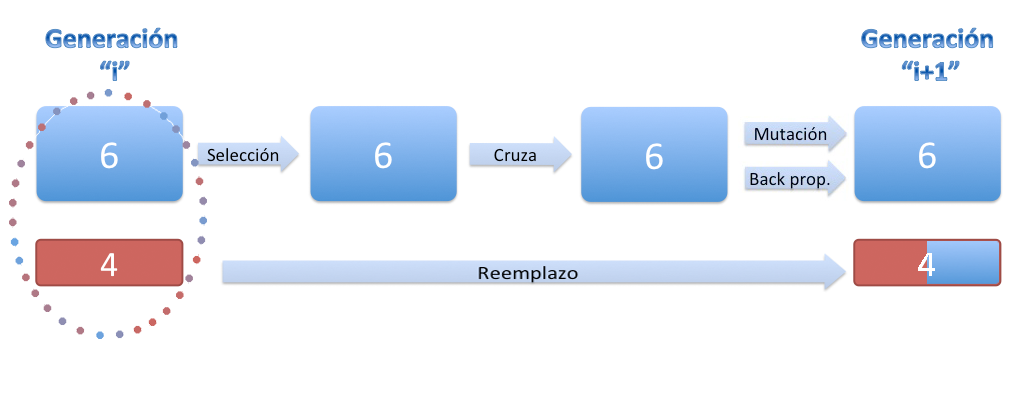
\includegraphics[scale=1.30]{./images/AlgGenModelado.png}
\label{modelado}
\end{center}
\end{figure}

\begin{center}
\par Figura 1: Modelado esquemático con N = 10 y G = 0.6.
\end{center}
\end{frame}

\subsection{Función de fitness}


\begin{frame}{Función de fitness}


\par La función de \textit{fitness} mide el grado de adaptación de un determinado individuo al entorno actual.

\begin{block}{Inversa del ECM}

\[
   f(i) = \frac{1}{ECM}
\]

Siendo:

\begin{itemize}
\item \textbf{i:} Red neuronal (individuo)
\item \textbf{ECM:} Error cuadrático medio obtenido al evaluar la red.
\end{itemize}
\end{block}


\end{frame}


\section{Métodos de selección y reemplazo}

\begin{frame}{Métodos de selección y reemplazo}
\par Los métodos de selección y reemplazo implementados son los siguientes:\\
\begin{itemize}
\item Ruleta
\item Boltzman
\item Elite
\item Universal
\item Mixto
\begin{itemize}
\item Elite + Ruleta
\item Elite + Boltzman
\end{itemize}
\end{itemize}
\end{frame}

\section{Criterios de corte}
\begin{frame}{Criterios de corte}

\par Los criterios de corte implementados son los siguientes:\\

\begin{itemize}
\item \textbf{Máxima cantidad de generaciones:} Dado un número $p$, el algoritmo termina al alcanzarse $p$ generaciones.
\item \textbf{Entorno al óptimo:} Se llega a la solución óptima o se alcanza un fitness superior a una determinada cota.
\end{itemize}
\end{frame}

\begin{frame}{Criterios de corte}
\begin{itemize}
\item \textbf{Contenido:} Se corta al detectar que el mejor fitness de la población no progresa con las generaciones.
\item \textbf{Estructura:} Se finaliza al detectar que una parte relevante de la poblacioón no cambia de generacioón en generación. Es decir, dado un porcentaje $p$, el algoritmo termina cuando la cantidad de individuos iguales de la generación es mayor a dicho $p$.
\end{itemize}
\end{frame}

\section{Mutación y backpropagation}
\begin{frame}{Mutación y backpropagation}

\par Una vez cruzados, los individuos pasan a la siguiente generación con una probabilidad baja de ser mutados y/o entrenados mediante \textit{backpropagation}.\\

\begin{itemize}
\item\textbf{Mutación:} Se toma un peso al azar del individuo y se le suma un número random proporcional al valor del mismo.
\end{itemize}
\end{frame}

\section{Resultados}
\begin{frame}{Resultados}

\begin{itemize}
\item A
\item B
\end{itemize}
\end{frame}


\section{Conclusiones}
\begin{frame}{Conclusiones}

\begin{itemize}
\item A
\item B
\end{itemize}

\end{frame}

\end{document}
